\section{$\epsilon$-constraint Method and CWMOIP}\label{sec:naiveSolutions}

When the problem size is relatively small, the $\epsilon$-constraint method and CWMOIP are two feasible methods to find the complete non-dominant solutions (a.k.a., true Pareto front).

\begin{algorithm}[t]
                  % enter the algorithm environment
\caption{Function \small{$EpsilonCont()$} for feature selection}\label{alg:naiveLP}
\small
    \KwIn{$M$: the feature model of the given system} %$maxIter$: the maximum number of iterations of the generation process
    %\KwIn{$userInfor$: the contextual information of user device} %$maxIter$: the maximum number of iterations of the generation process
    \KwOut{$solutions$: a non-dominated solution set for feature selection}
    %\KwOut{$returnedSol$: a solution returned to guide malware generation }
    $E~\leftarrow~\emptyset$\;\label{algo:lp:i1}
    $f^{TUB}_2 = getObjTheoBound(M,\mathcal{F}_2), f^{TLB}_2 = 0$\;\label{algo:lp:i2}
    $f^{TUB}_3 = getObjTheoBound(M,\mathcal{F}_3), f^{TLB}_3 = 0 $\;\label{algo:lp:i3}
    $f^{TUB}_4 = getObjTheoBound(M,\mathcal{F}_4), f^{TLB}_4 = 0 $\;\label{algo:lp:i4}

     \For{$ p=f^{TLB}_2;   p \le f^{TUB}_2; p = p \small{+} 1$}{\label{algo:lp:f1}
        \For{$ q= f^{TLB}_3;  q \le f^{TUB}_3; q = q\small{+} 1$}{\label{algo:lp:f2}
          \For{$ t=f^{TLB}_4;  t \le f^{TUB}_4; t = t\small{+} 1$}{\label{algo:lp:f3}
          %$conj(\mathcal{F}_2) = convert(\mathcal{F}_2,p) $\; \label{algo:lp:lp1}
          %$conj(\mathcal{F}_3) = convert(\mathcal{F}_3,q) $\; \label{algo:lp:lp2}
          %$conj(\mathcal{F}_4) = convert(\mathcal{F}_4,t) $\; \label{algo:lp:lp3}
          $allCons= conj(M) \cup \{\mathcal{F}_2\le p\} \cup \{\mathcal{F}_3\le q\}  \cup \{\mathcal{F}_4 \le t\} $\;\label{algo:lp:lp4}
          $ME = bintprog(allCons,\mathcal{F}_5) $\; \label{algo:lp:lp5}
          $E = E \cup ME$\;  \label{algo:lp:lp6}
          }
        }
     }
    % $returnedSol = solutions.First()$\;
   %  \For{$sol  \in  nondominatedSol$}{  \label{algo:lp:f3}
%        \If {$  aggregatedObj(sol) < aggregatedObj(returnedSol)$} {               \label{algo:lp:if1}
%       %  \If {$ satisfyExtraConst(sol) == true $} {               \label{algo:lp:if2}
%          $returnedSol = sol$\; \label{algo:lp:if3}
%       %   }
%        }
%     }

    \KwRet $E$;\label{algo:lp:rt}
      %  $allMal\leftarrow allMal \cup newGeneration$\;\label{algo:cmb:23}

\end{algorithm}

\subsection{$\epsilon$-constraint Method}
The idea is to make $k-1$ objectives as the range constraints and use the $k$-th one as the objective function in BIP \cite{e-constraint}. As \emph{obj1} is correctness, in BIP, all the constraints are satisfied, \emph{obj1} is always 0 in theory and thus $\mathcal{F}_1(\vec x)$ is not needed. So $\mathcal{F}_2(\vec x)$, $\mathcal{F}_3(\vec x)$, $\mathcal{F}_4(\vec x)$ can be converted to range constraints. Each range constraint's upper bound will be iterated from 0 to the upper bound of the corresponding objective, by step size 1.

The detailed procedures are shown in Algorithm \ref{alg:naiveLP}. Note that $getObjTheoBound(M,\mathcal{F}_2)$ at line \ref{algo:lp:i2} finds the theoretic upper bound $f^{TUB}_2$ for $\mathcal{F}_2$ --- for \emph{JCS}, it is 12 when all $x_i=0$  and $conj(M)$ is not considered. Similarly, $f^{TUB}_3$ and $f^{TUB}_4$ are $\sum\nolimits_{i=1}^{n}a_i$ and $\sum\nolimits_{i=1}^{n}b_i$ respectively,  when the size of feature set $n = \mathit{\vert Fea(JCS) \vert} =12$ for \emph{JCS}. At line \ref{algo:lp:lp4},  $allCons$ is the union of the original inequalities of the formula (\ref{formula:mop}) and three new inequalities converted from other constrained objectives in formula  (\ref{formula:singLP}). At line \ref{algo:lp:lp5}, $bintprog(allCons,\mathcal{F}_5)$ calls the BIP function for objective $\mathcal{F}_5$ such that $allCons$ are satisfied.

\vspace{-3mm}
\begin{equation}\label{formula:singLP}
%%\begin{array}{rrclcl}
%%\displaystyle \min_{x} & \multicolumn{3}{l}{c^T x} \\
%%\textrm{s.t.} & A x & \geq & b \\
%%%&\displaystyle \sum_{i=0}^{n} x_i & = & 1 \\
%%& x_i & \in & \{0,1\} & & \forall i \in \{1...n\} \\
\begin{array}{ll@{}r@{}r@{}l}
     \text{Min} & \mathcal{F}_5(\vec x) =\sum\nolimits_{i=1}^{n}(c_i\cdot x_i) \\[\jot]
     \text{s.t.} & \sum\nolimits_{i=1}^{n}(1-x_i) \le p \\[\jot]
      & \sum\nolimits_{i=1}^{n}(a_i\cdot x_i) \le q \\[\jot]
      & \sum\nolimits_{i=1}^{n}(b_i\cdot x_i) \le t\\[\jot]
       & \text{the inequalities for $conj(M)$ hold}\\[\jot]
%    &  x_1 - x_3  \ge 0   \\
%    &  x_1 - x_4 \ge 0      \\
%    &  x_1 - x_5 \ge 0      \\
%    &  x_1 - x_6 \ge 0      \\
%    &  x_1 - x_7 \ge 0      \\
%    &  x_2 - x_8 \ge 0      \\
%    &  x_2 - x_9 \ge 0      \\
%    &  x_2 - x_{10} \ge 0      \\
%    &  -x_2 + x_8 + x_9 + x_{10}\ge 0      \\
%    &  -x_8 - x_9 - x_{10}\ge -1      \\
%    &  x_6 - x_{11} \ge 0      \\
%    &  x_6 - x_{12} \ge 0      \\
%    &  -x_6 + x_{11} + x_{12} \ge 0      \\
%    &  x_7 - x_{11} \ge 0      \\
%    &  x_7 - x_{12} \ge 0      \\
%    &  -x_7 + x_{11} + x_{12} \ge 0      \\
  \end{array}
\vspace{-3mm}
%%\end{array}
\end{equation}

Algorithm \ref{alg:naiveLP} is of the time complexity of $O(n^3)$, if considering BIP solving function $bintprog()$ takes constant time --- a time limit is set in its practical usage. Solving the MOBIP problem in formula (\ref{formula:mop}) is reduced to solving the BIP problem in formula (\ref{formula:singLP}) by many times --- precisely, it is a number of $(n+1)  ({\sum\nolimits_{i=1}^{n}a_i}+1)({\sum\nolimits_{i=1}^{n}b_i}+1)$ times.



\subsection{CWMOIP}
CWMOIP, proposed by  \"{O}zlen \emph{et al.}~\cite{DBLP:journals/eor/OzlenA09}, is an objective-reduction technique for MOIP. CWMOIP is for generating \emph{all} non-dominant solutions.
It improves the $\epsilon$-constraint method by two steps: (1) for each objective, the lower bound is not 0 and the upper bound is not the sum of feature attributes revelent to that objective. To be precise, BIP is applied to get the true lower and upper bounds for each objective (i.e., $\mathcal{F}_2$ to $\mathcal{F}_5$) separately, subject to the  conjunction of constraints $conj(M)$. (2) objective-reduction is implemented via the constraint weight method, to avoid generating dominant solutions. The $k$-objective problem is first reduced to that of $k-1$, then $k-2$, iteratively, until the last objective.

\noindent\textbf{Example for (1).} In the precise calculation of the upper and lower bounds, for the example of \emph{JCS} with 12 features, the true bounds $f^{LB}_2$ and $f^{UB}_2$ for $\mathcal{F}_2(\vec x)$ are 2 (a maximum of 10 selected  features) and 9 (a minimum of 3 selected) respectively, not 0 and 12 in the $\epsilon$-constraint method. Hence, in $\epsilon$-constraint method 13 (12-0+1) times of iteration is needed for the outermost loop at line~\ref{algo:lp:f1} in Algorithm \ref{alg:naiveLP}, while  only 8 (9-2+1) times is needed for CWMOIP.


\begin{algorithm}[t]                  % enter the algorithm environment
\caption{Function \small{\emph{CWMOIP()}} for $k$-objective IP}\label{alg:cwmoip}
\small
    %\KwIn{$M$: the feature model of the given system} %$maxIter$: the maximum number of iterations of the generation process
    \KwIn{$k$: the number of objectives, $l_k$: constrained value for the weighted $k$-th \emph{obj}, $X$: the set of linear constraints}
    %\KwIn{$userInfor$: the contextual information of user device} %$maxIter$: the maximum number of iterations of the generation process
    \KwOut{$E$: the set of non-dominant solutions}
    %\KwOut{$returnedSol$: a solution returned to guide malware generation }
    $E~\leftarrow~\emptyset$\;\label{algo:cwmoip:i1}
    $f^{UB}_2,f^{LB}_2  = getObjTrueBound(X,f_2)$\;\label{algo:cwmoip:i2}
    $ ...$//get true bounds for other objective $3$ to $k-1$\;\label{algo:cwmoip:i3}
      $f^{UB}_k,f^{LB}_k  = getObjTrueBound(X,f_k)$\;\label{algo:cwmoip:i4}
      $w_k =\frac{1}{(f^{UB}_2-f^{LB}_2+1)(f^{UB}_3-f^{LB}_3+1)...(f^{UB}_k-f^{LB}_k+1)}$ \;\label{algo:cwmoip:i5}
    %   $l_k = f^{UB}_k$\;\label{algo:cwmoip:65}
      \If{$ k =1$}{\label{algo:cwmoip:i6}
           $E =E \cup bintprog(X,f_k)$ \;\label{algo:cwmoip:i6:if1}
       }
     \While{$true$}{\label{algo:cwmoip:f1}
         $ f_1 = addObjFuncSuffix(f_1,w_k \cdot f_k ) $\;\label{algo:cwmoip:f2}
         $ X^\prime = X \cup \{f_k \le l_k\}$\;\label{algo:cwmoip:f3}
         $ ME= CWMOIP(k-1,l_k,X^\prime) $ \;\label{algo:cwmoip:f4}
         \If{$ME = Null \empty$ }{\label{algo:cwmoip:f5}
             $break$\;\label{algo:cwmoip:if2}
         }
          $   E = E \cup ME$\;\label{algo:cwmoip:f6}
         $l_k = Max(f_k(\vec x),\vec x \in ME) -1$\;\label{algo:cwmoip:f7}

     }
    % $returnedSol = solutions.First()$\;
   %  \For{$sol  \in  nondominatedSol$}{  \label{algo:lp:f3}
%        \If {$  aggregatedObj(sol) < aggregatedObj(returnedSol)$} {               \label{algo:lp:if1}
%       %  \If {$ satisfyExtraConst(sol) == true $} {               \label{algo:lp:if2}
%          $returnedSol = sol$\; \label{algo:lp:if3}
%       %   }
%        }
%     }

    \KwRet $E$;\label{algo:cwmoip:rt}
      %  $allMal\leftarrow allMal \cup newGeneration$\;\label{algo:cmb:23}

\end{algorithm}



\begin{figure}[t]
\vspace{-5.5mm}
\centering
%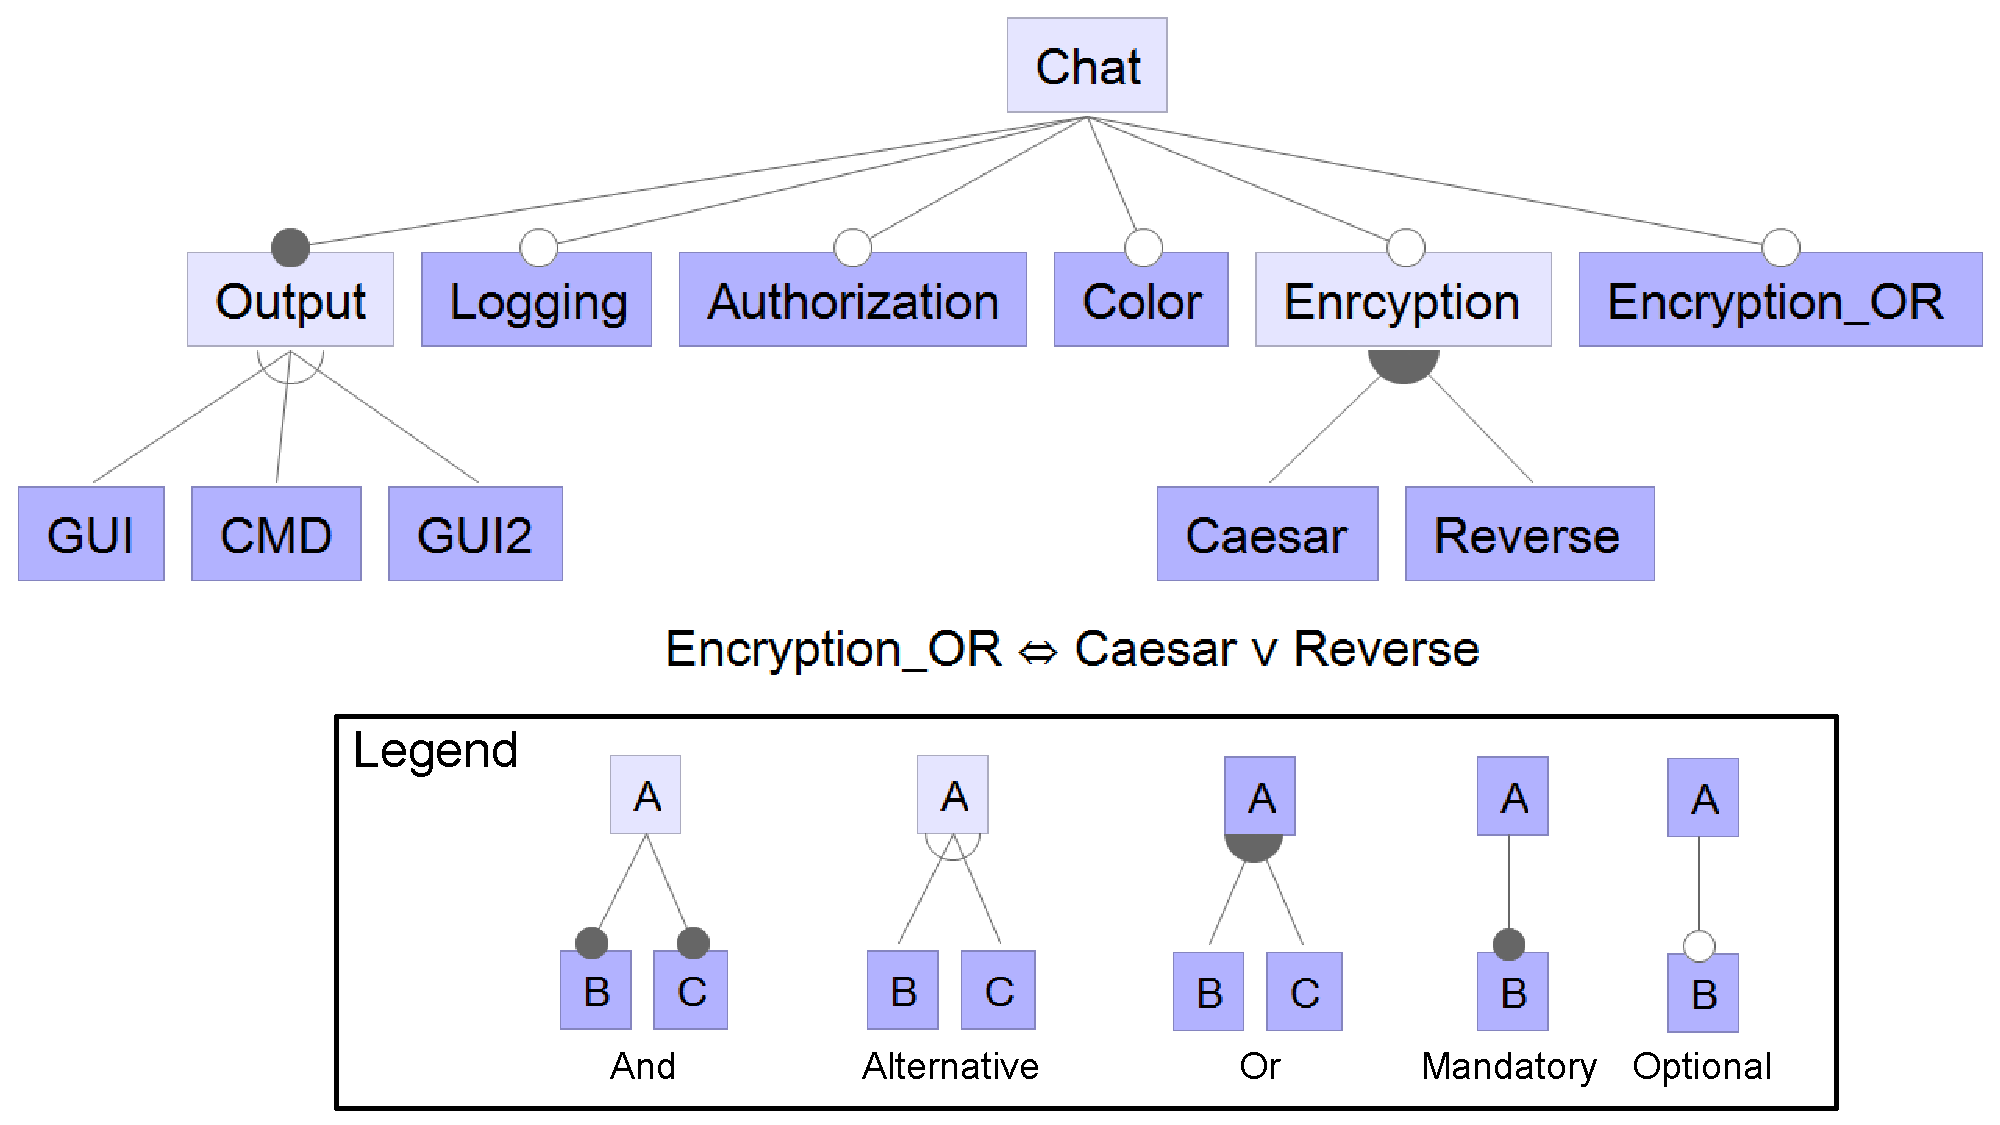
\epsfig{file=image/fm.bmp, width=8.5cm}
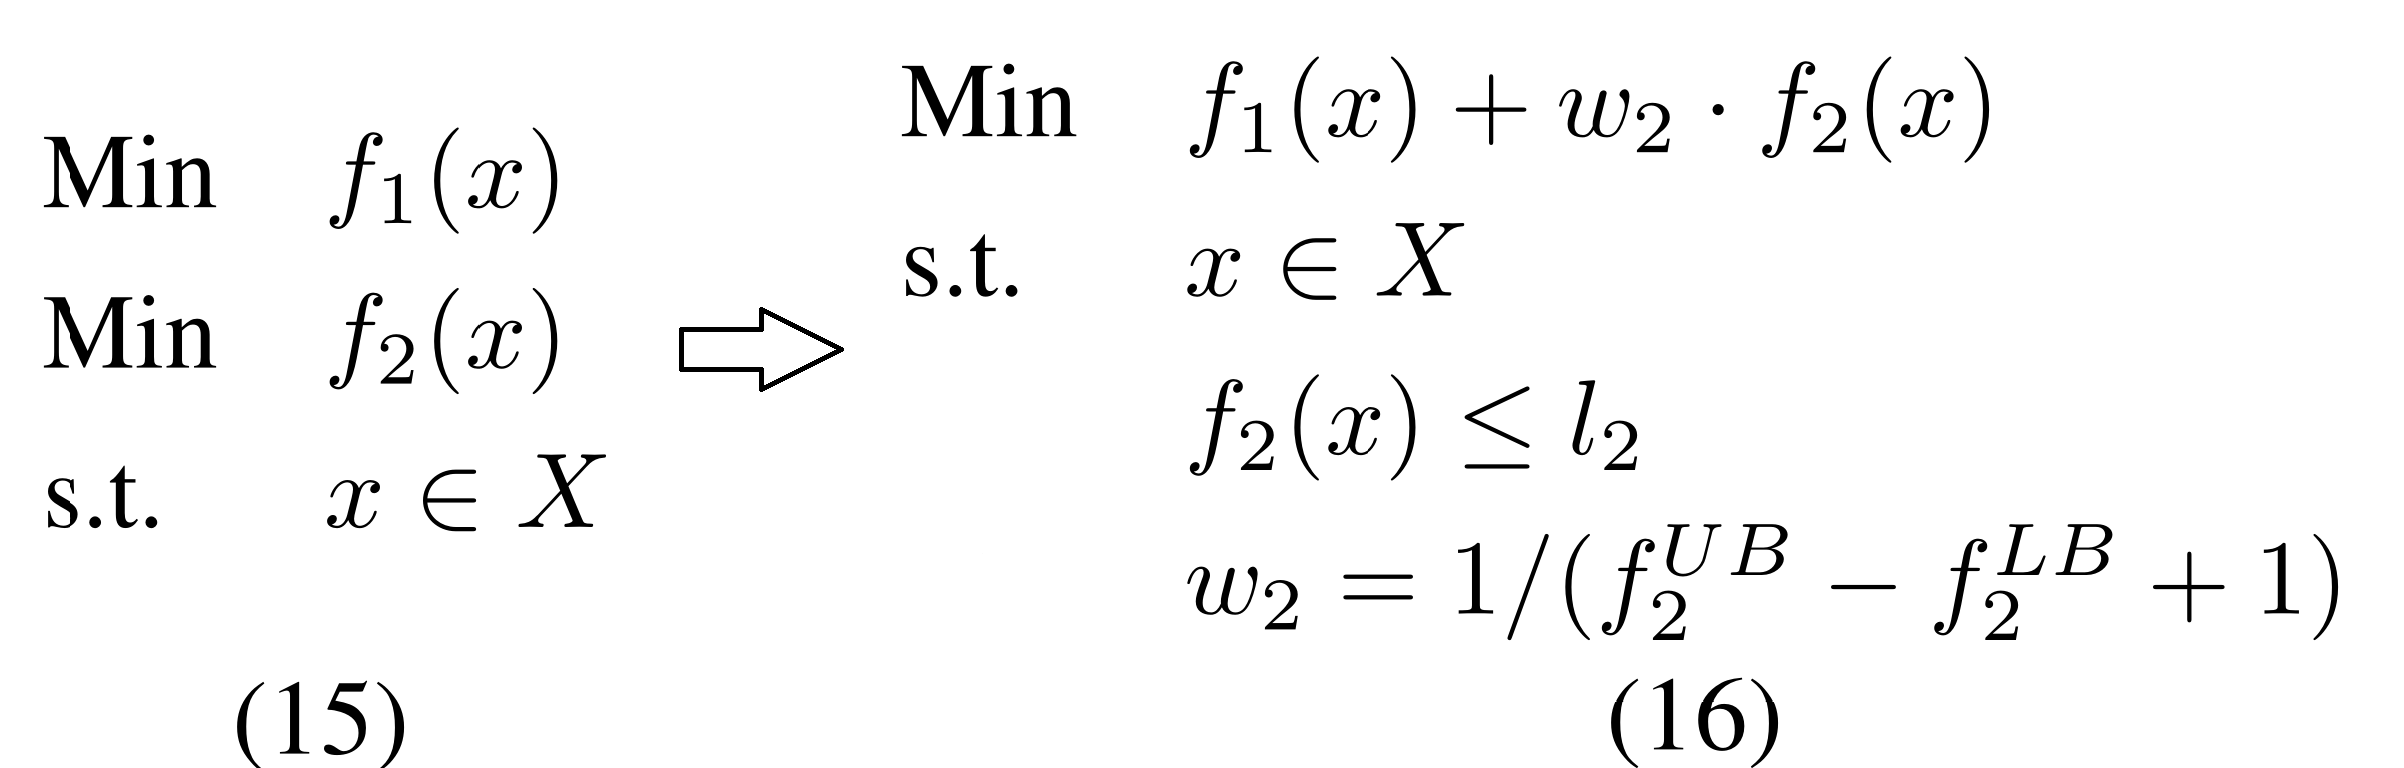
\includegraphics[width=7.8cm]{image/CWMOIP.png}
\vspace{-3.5mm}
\caption{An example of applying CWMOIP for a $bi$-objective problem}
\label{fig:cwmoip_exam}
\end{figure}


\noindent\textbf{Example for (2).}  Fig.~\ref{fig:cwmoip_exam} shows an example for objective-reduction. Solving the $bi$-objective problem in formula (15)  is reduced to solving the 1-objective problem in formula (16) by \rev{$l_2$} times. It is named "constraint weighted" because of the weight $w_2$ and the constraint $ f_2(x) \le l_2$. %on the original objective $ f_2(x)$.
 Variable $l_2$ iterates from the lower bound $f^{LB}_2$ to the upper bound $f^{UB}_2$ of $ f_2(x)$. %Here, $f^{LB}_2$ (or $f^{UB}_2$) denotes the lower (or upper) bound  of $ f_2(x)$.}
%Interested readers can refer to \cite{DBLP:journals/eor/OzlenA09} for the details of the proof.



In Algorithm \ref{alg:cwmoip}, we show the general steps of finding all non-dominant solutions for any given $k$-objective BIP problem~\cite{DBLP:journals/eor/OzlenA09} (not limited to the model of our problem). The initial invocation of Algorithm \ref{alg:cwmoip} is calling $CWMOIP(k,f^{UB}_k,X)$, and then $CWMOIP(k-1,l_k,X)$ at line \ref{algo:cwmoip:f4}, recursively, until calling $CWMOIP(1,l_2,X)$. %We explain the important steps in Algorithm 2.
Initially, lines \ref{algo:cwmoip:i2} to \ref{algo:cwmoip:i4} calculate the true upper and lower bounds of the $2$-nd objective to the $k$-th, subject to the constraint set $X$ (In practice, this can be done once and results are cached for reuse). Then $w_k$ is calculated for the $k$-th objective at line \ref{algo:cwmoip:i5}. In the loop at line \ref{algo:cwmoip:f1}, the $k$-objective problem is reduced to a new \emph{(k-1)}-objective problem (line \ref{algo:cwmoip:f4}), which has the new suffix $w_k\cdot f_k(\vec x)$ for the objective function (line \ref{algo:cwmoip:f2}) and the new constraint $f_k(\vec x) \le l_k$ for the constraint set $X$ (line \ref{algo:cwmoip:f3}). If no results are found (lines \ref{algo:cwmoip:f5}-\ref{algo:cwmoip:if2}), the recursion process stops. If found, the constraint $l_k$ is tightened to the value just smaller than the largest value of  $f_k(\vec x)$ for $\vec x \in ME$. Last, BIP solving function is called when only one objective ($k=1$) is left at line \ref{algo:cwmoip:i6} to \ref{algo:cwmoip:i6:if1}.

According to \cite{DBLP:journals/eor/OzlenA09}, the maximum number of recursion is $\frac{|E|(|E|+1)...(|E|+k-2)}{2\cdot 3 \cdot ... \cdot(k-1)}$.
Note that in our example, $\mathcal{F}_1(\vec x)$ is not needed as it is always   $0$ for BIP. Thus, it is a 4-objective ($\mathcal{F}_2(\vec x)$ to $\mathcal{F}_5(\vec x)$) BIP problem. $CWMOIP()$ will reduce it to constrain-weighted 3-objective ($\mathcal{F}_2(\vec x)$ to $\mathcal{F}_4(\vec x)$); iteratively, until to a constrain-weighted 1-objective ($\mathcal{F}_2(\vec x)$) problem.
%\begin{equation}\label{formula:singLP}
%%%\begin{array}{rrclcl}
%%%\displaystyle \min_{x} & \multicolumn{3}{l}{c^T x} \\
%%%\textrm{s.t.} & A x & \geq & b \\
%%%%&\displaystyle \sum_{i=0}^{n} x_i & = & 1 \\
%%%& x_i & \in & \{0,1\} & & \forall i \in \{1...n\} \\
%\begin{array}{ll@{}r@{}r@{}l}
%     \text{Min} & f_1(x) \\[\jot]
%     \text{Min} & f_2(x) \\[\jot]
%     \text{s.t.}& x \in X\\[\jot]
%  \end{array}
%\vspace{-3mm}
%%%\end{array}
%\end{equation}
%
%%\subsection{Preliminary Evaluation Results}
%\begin{equation}\label{formula:singLP}
%%%\begin{array}{rrclcl}
%%%\displaystyle \min_{x} & \multicolumn{3}{l}{c^T x} \\
%%%\textrm{s.t.} & A x & \geq & b \\
%%%%&\displaystyle \sum_{i=0}^{n} x_i & = & 1 \\
%%%& x_i & \in & \{0,1\} & & \forall i \in \{1...n\} \\
%\begin{array}{ll@{}r@{}r@{}l}
%     \text{Min} & f_1(x) + w_2 \cdot f_2(x)\\[\jot]
%     \text{s.t.} &  x \in X \\[\jot]
%     \text{s.t.}& f_2(x) \le l_2\\[\jot]
%     \text{s.t.}& w_2 = 1 / (f^{UB}_2-f^{LB}_2+1) \\[\jot]
%  \end{array}
%\vspace{-3mm}
%%%\end{array}
%\end{equation}
%
